% !TEX root = ../main.tex
%% ---------------------------------------------------------------------------
% 4.4 2D manufactured plate
%% ---------------------------------------------------------------------------

\subsection{2D manufactured plate}\label{sec:manufactured2d}

As shown in Fig. \ref{fig:21}, we perform the assessment of convergence performance on a manufactured plate, whose material and geometric properties are $D=2\times10^{4}$, Poisson's ratio $\nu=0.3$, length $L=10$.
The manufactured solution is state as:
\begin{equation}\label{plate_manufactured}
w=\left(x+2y+1\right)^{8}/1000
\end{equation}

\begin{figure}[pos=htbp]
\centering
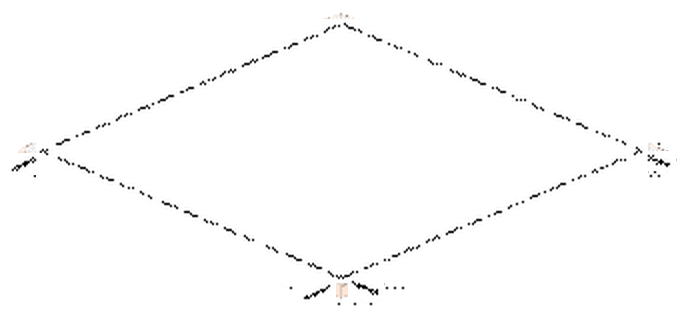
\includegraphics[width=0.6\textwidth]{figs/fig21.png}
\caption{Description of 2D manufactured plate.}\label{fig:21}
\end{figure}

The same as Section \ref{sec:quadratic}, five regular grids with 36, 121, 441, 1681, and 6561 nodes are applied to discrete the 2D domain.
The corresponding results are listed in Figs. \ref{fig:22}--\ref{fig:27}, which clearly evince that, with the reduce of nodal distance, the convergence rates of Gauss integration based method constantly deteriorate until reach the theoretical values, which are far below the optimal ones.
However, no matter which order of basis function is adopted, the convergence rates of RKGSI always keep $(p+1)$, $p$ and $(p-1)$, regarding the $L_2$, $H_1$ and $H_2$ error norms.

\begin{figure}[pos=htbp]
\centering
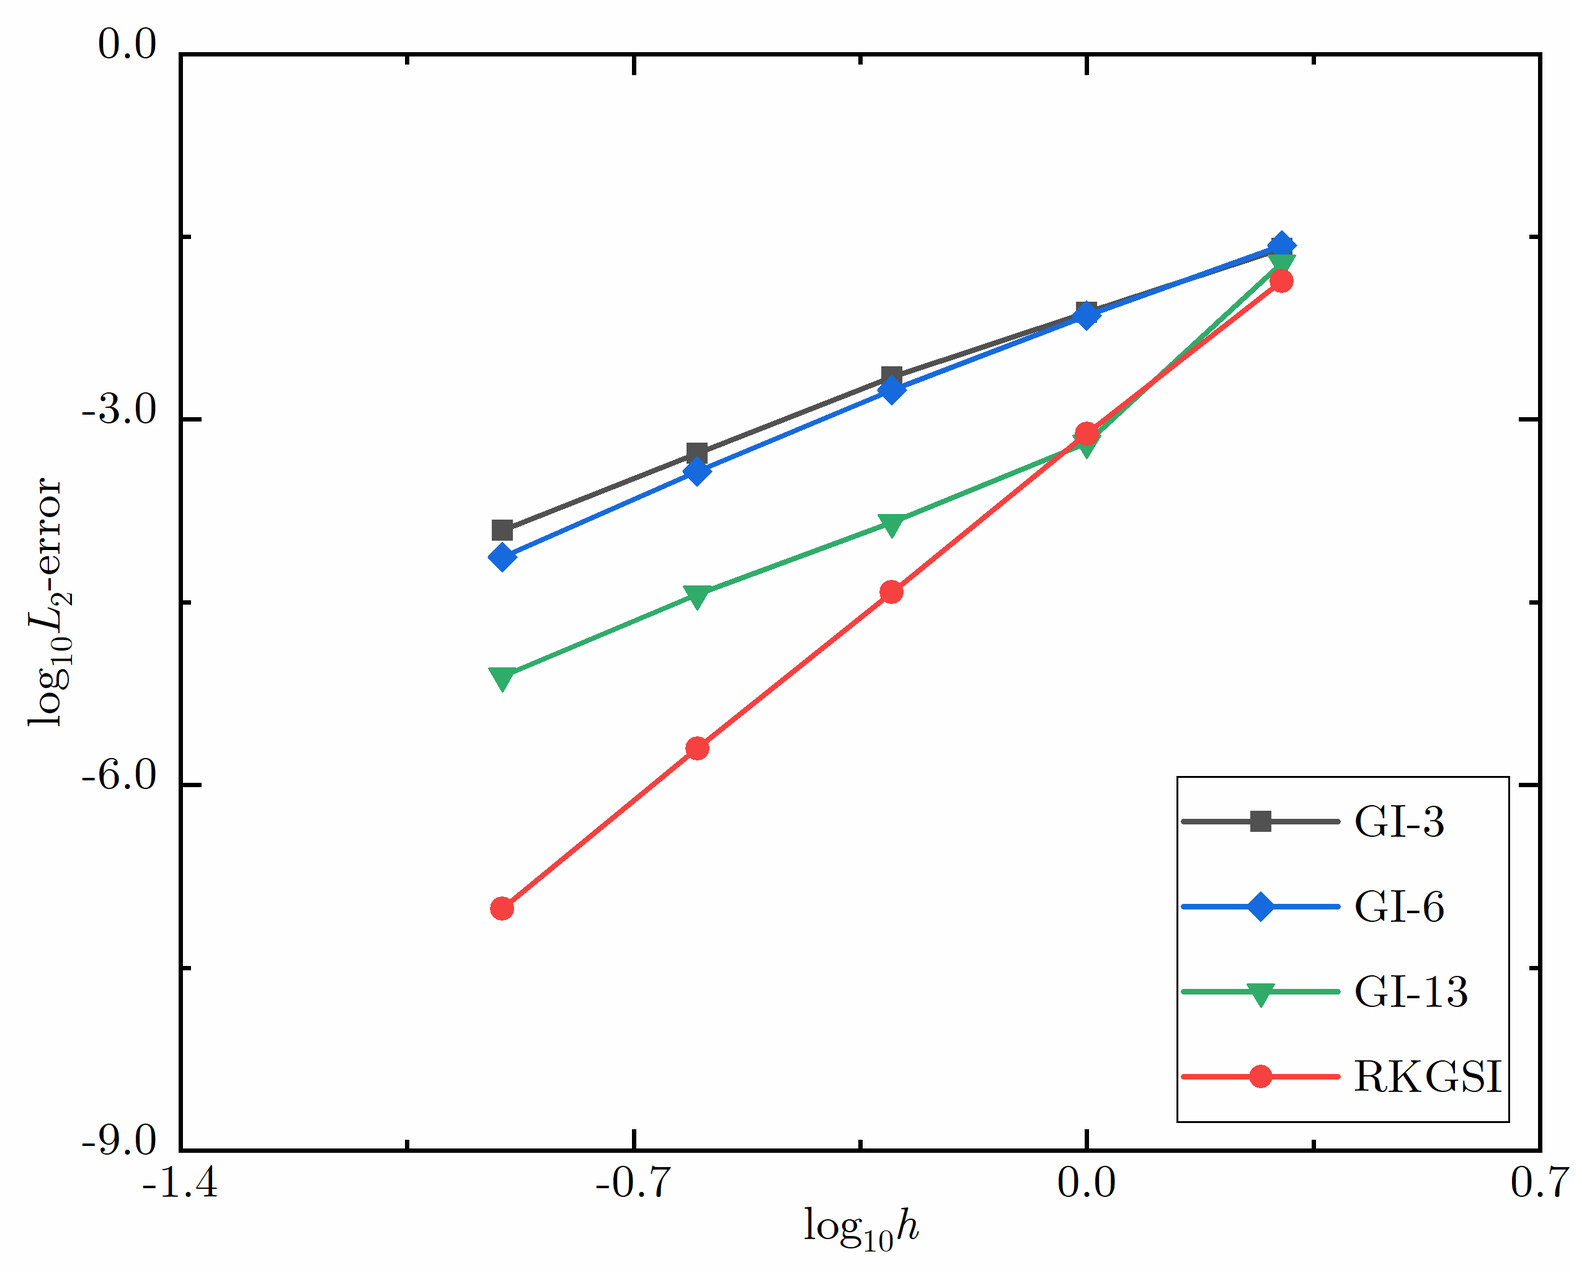
\includegraphics[width=0.55\textwidth]{figs/fig22.png}
\caption{$L_2$-error comparison for the 2D manufactured plate with $p=3$.}\label{fig:22}
\end{figure}

\begin{figure}[pos=htbp]
\centering
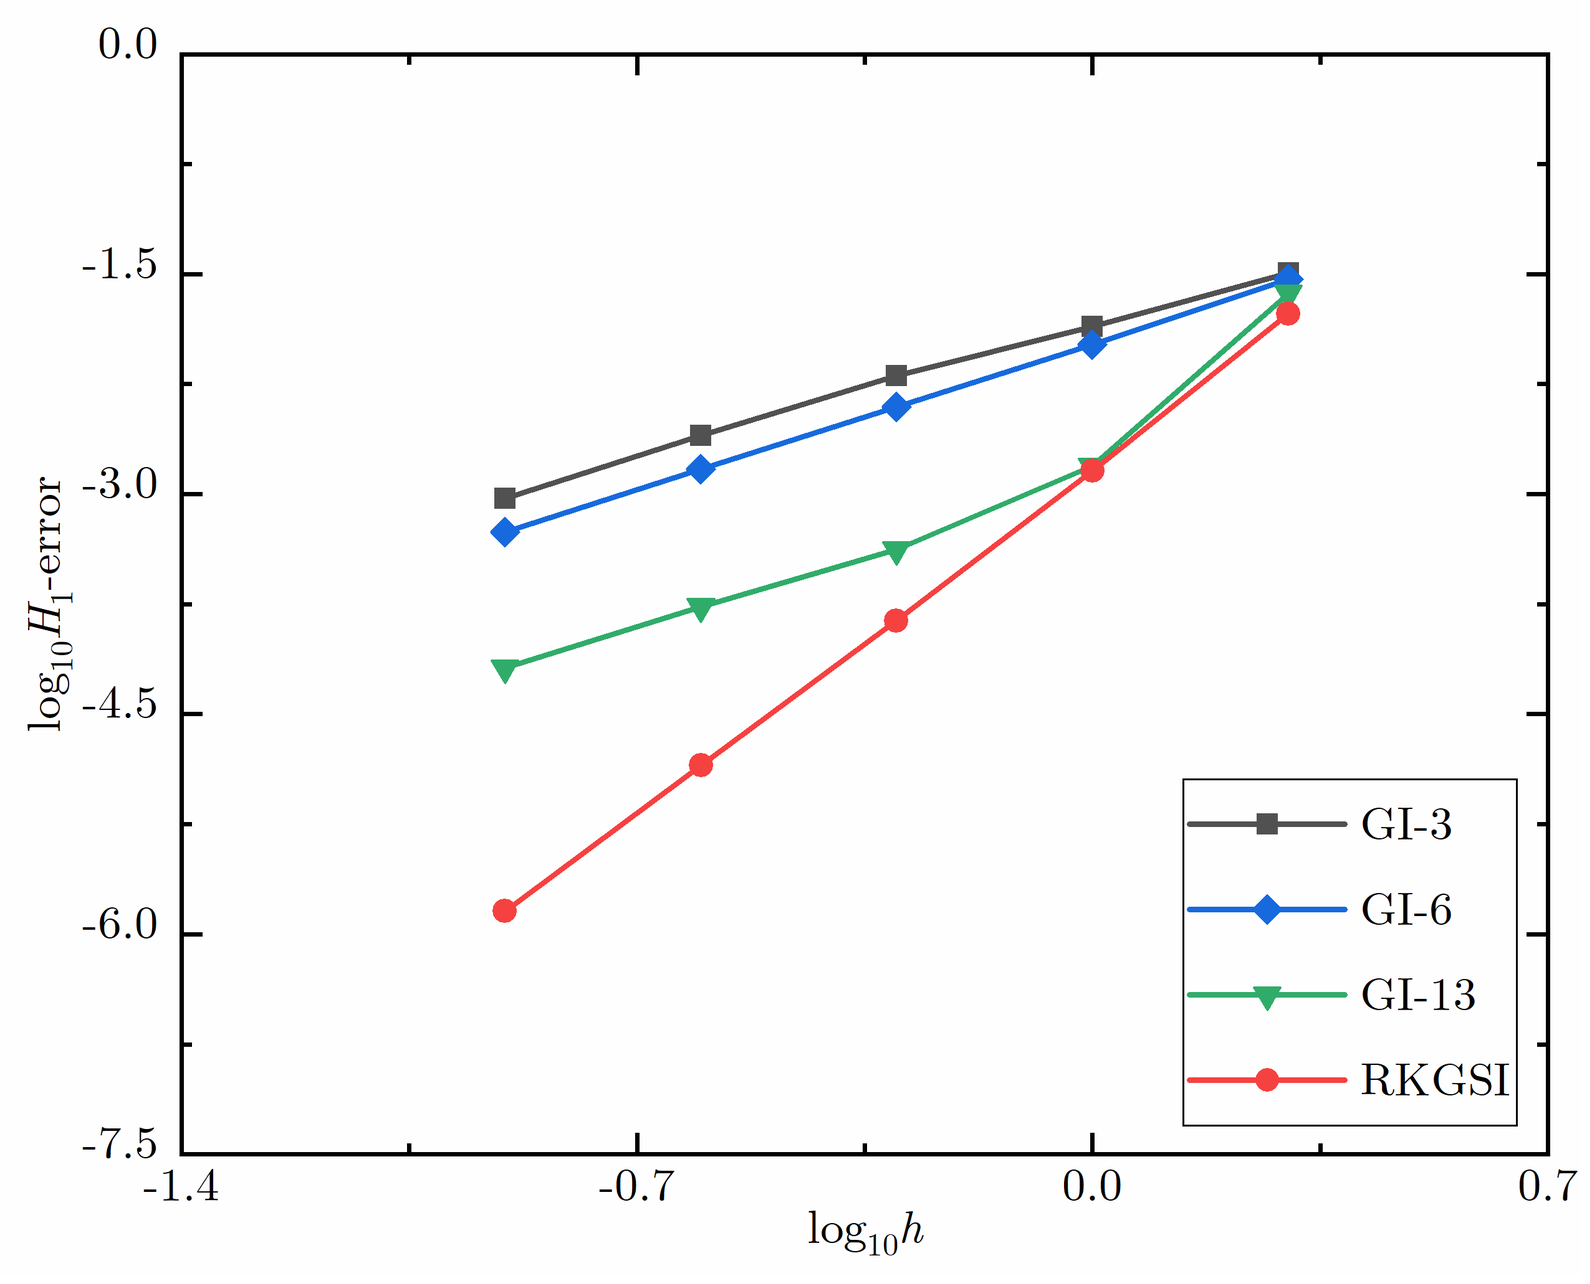
\includegraphics[width=0.55\textwidth]{figs/fig23.png}
\caption{$H_1$-error comparison for the 2D manufactured plate with $p=3$.}\label{fig:23}
\end{figure}

\begin{figure}[pos=htbp]
\centering
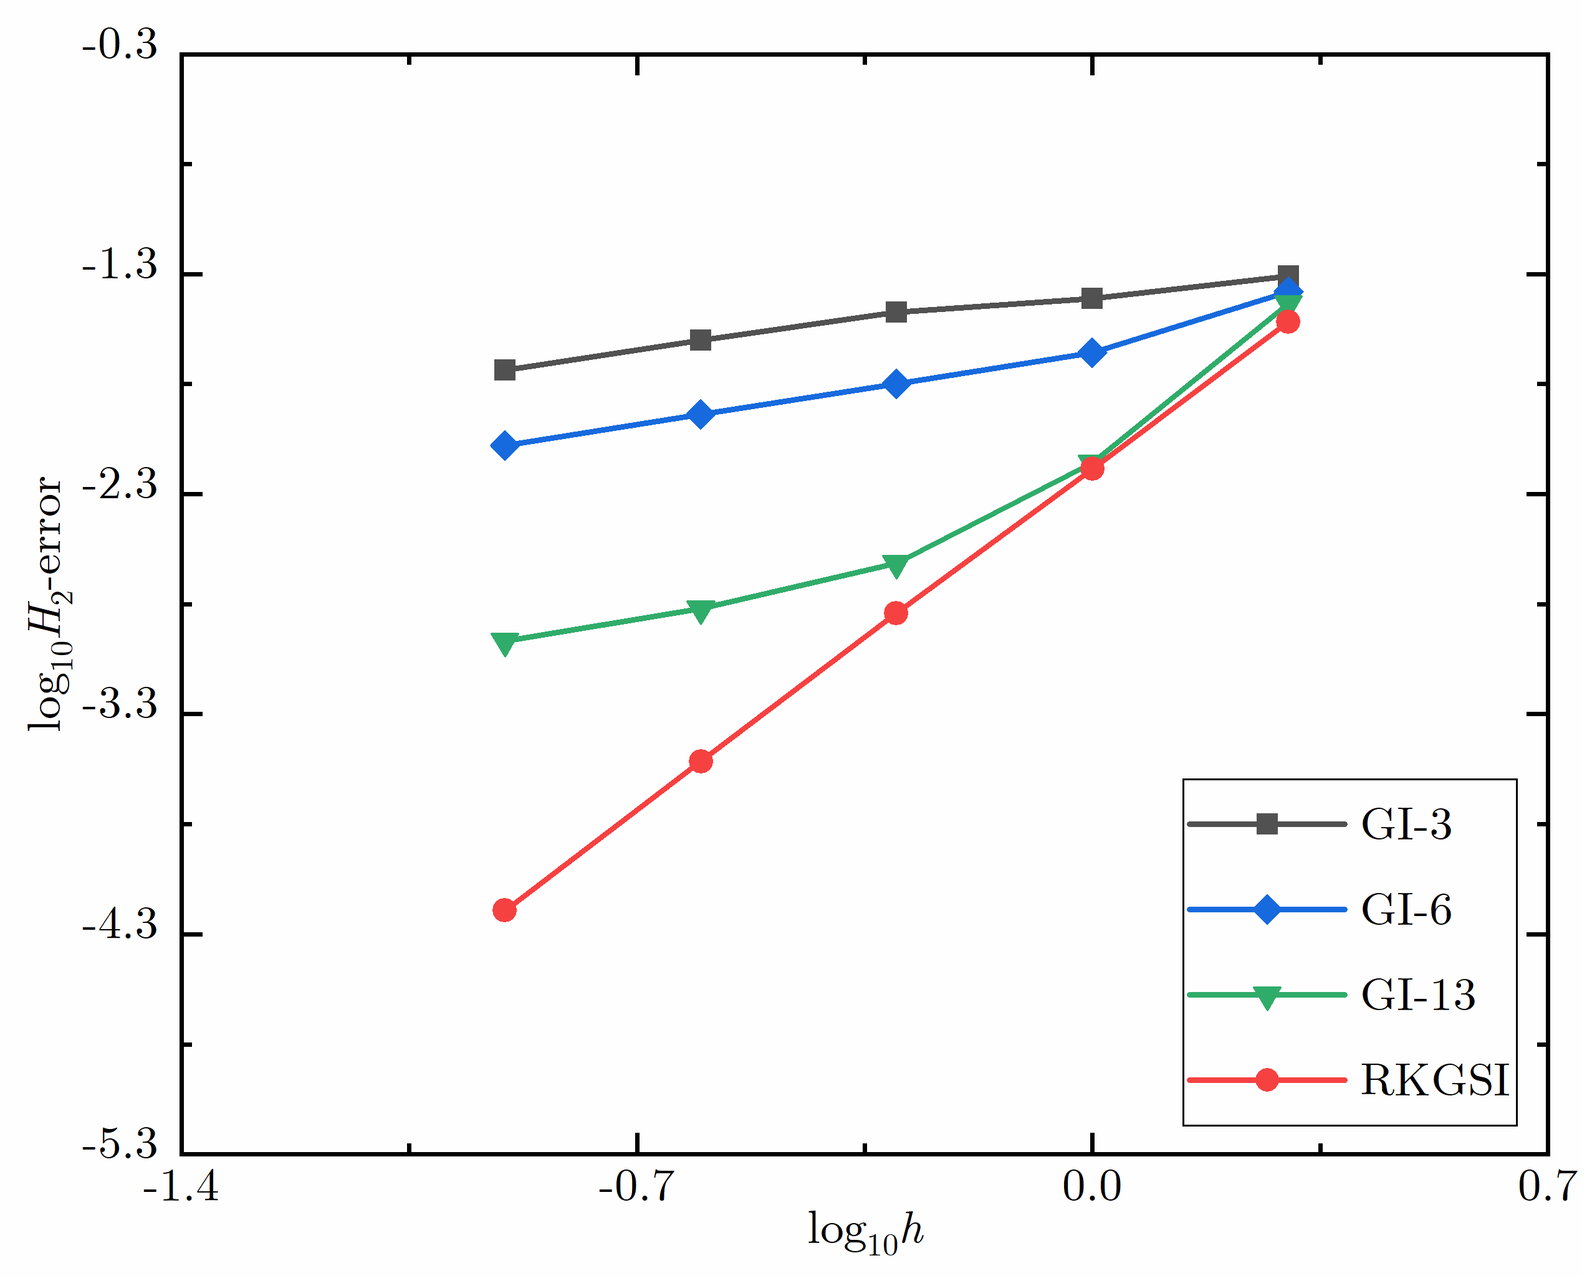
\includegraphics[width=0.55\textwidth]{figs/fig24.png}
\caption{$H_2$-error comparison for the 2D manufactured plate with $p=3$.}\label{fig:24}
\end{figure}

\begin{figure}[pos=htbp]
\centering
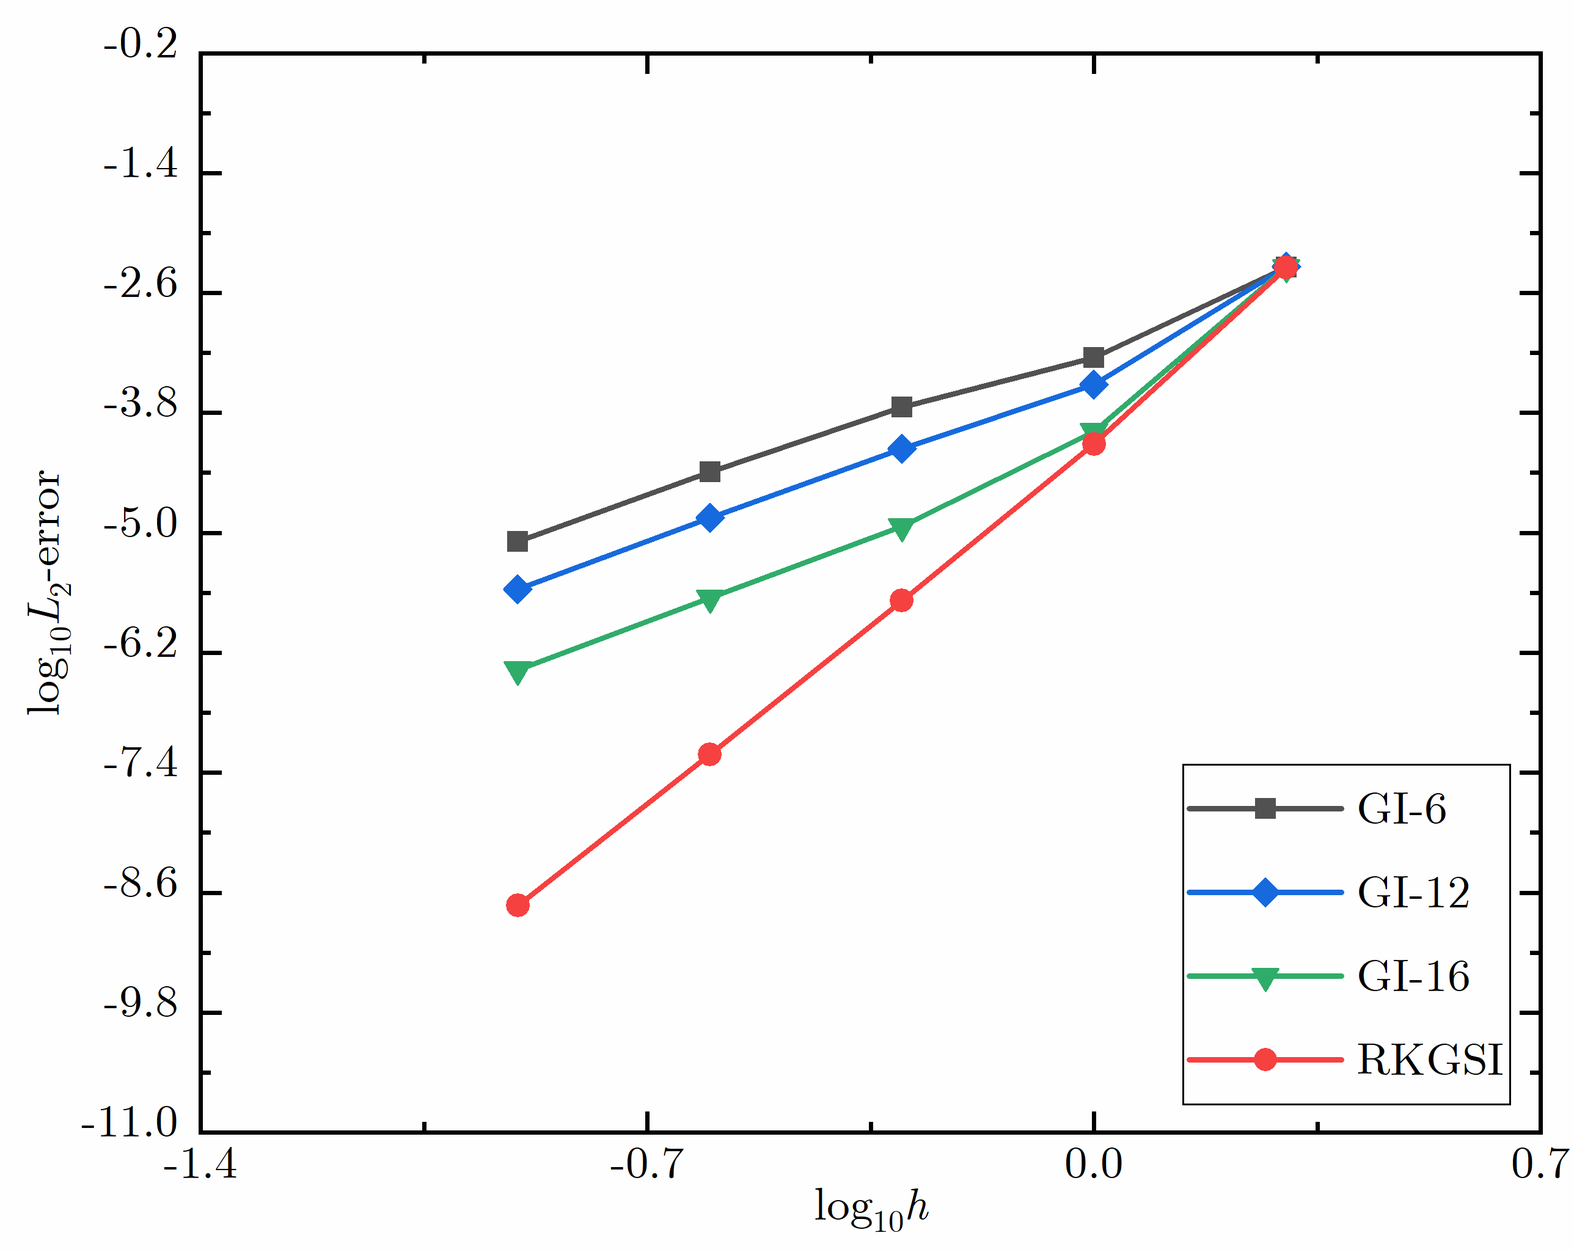
\includegraphics[width=0.55\textwidth]{figs/fig25.png}
\caption{$L_2$-error comparison for the 2D manufactured plate with $p=4$.}\label{fig:25}
\end{figure}

\begin{figure}[pos=htbp]
\centering
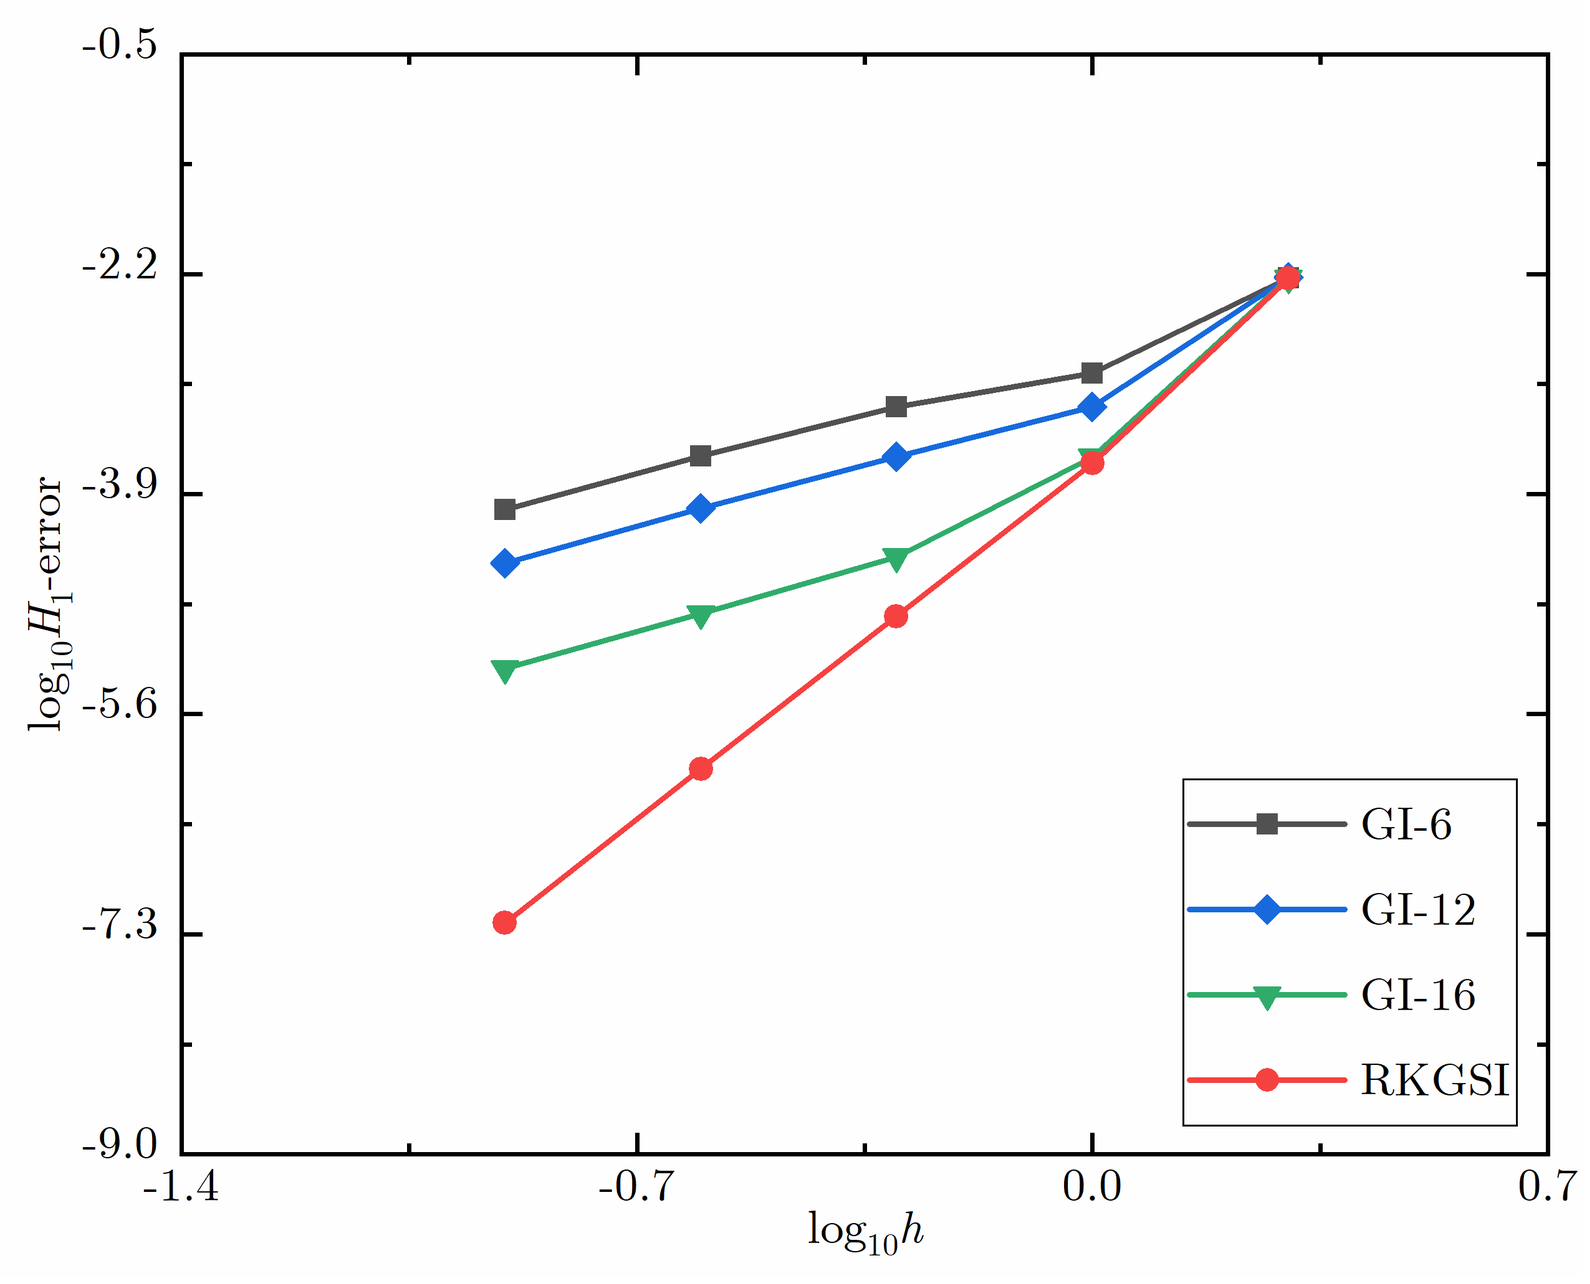
\includegraphics[width=0.55\textwidth]{figs/fig26.png}
\caption{$H_1$-error comparison for the 2D manufactured plate with $p=4$.}\label{fig:26}
\end{figure}

\begin{figure}[pos=htbp]
\centering
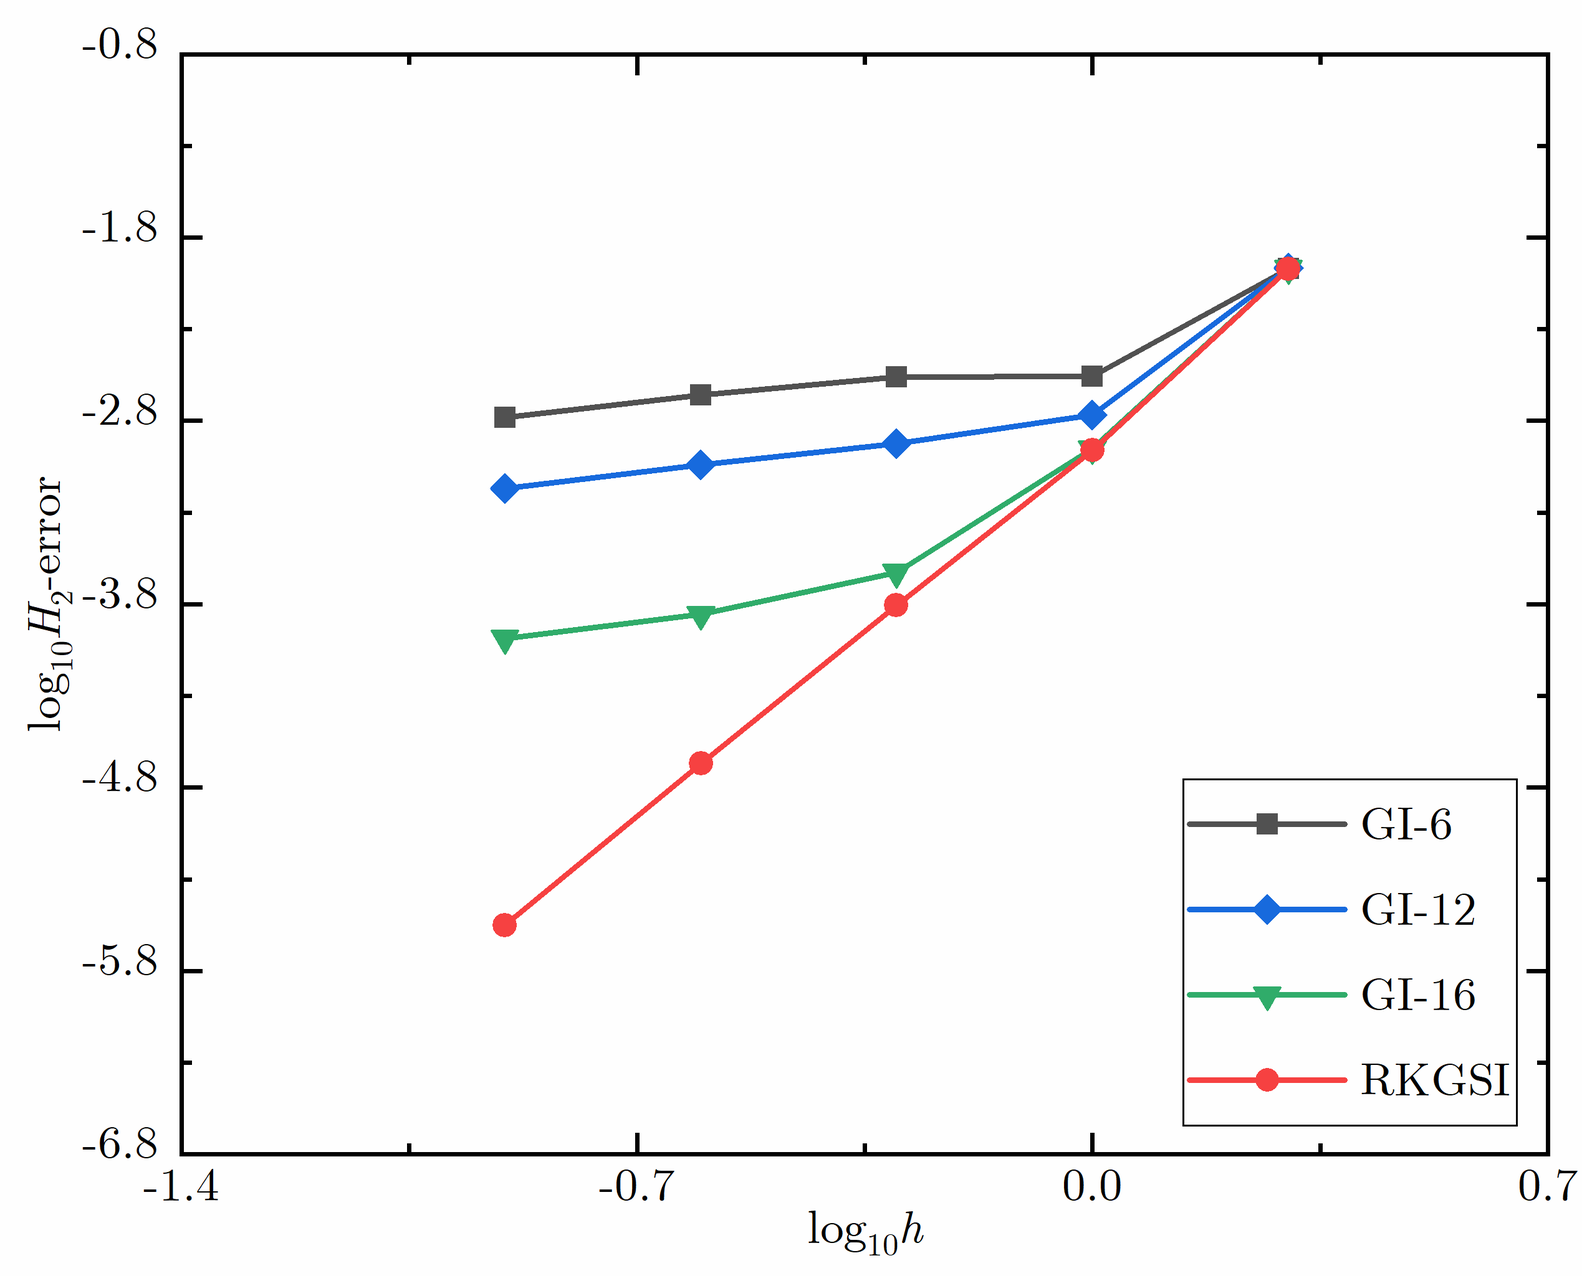
\includegraphics[width=0.55\textwidth]{figs/fig27.png}
\caption{$H_2$-error comparison for the 2D manufactured plate with $p=4$.}\label{fig:27}
\end{figure}
